\documentclass[nobib]{tufte-handout}
\usepackage[utf8]{inputenc}
\usepackage[english]{babel}

\title{nbinteract: Generate Interactive Web Pages From Jupyter Notebooks}

\author[Samuel Lau]{Samuel Lau}

%\date{28 March 2010} % without \date command, current date is supplied

%\geometry{showframe} % display margins for debugging page layout

\usepackage[
  backend=bibtex,
  style=numeric,
  citestyle=numeric
]{biblatex}
\addbibresource{thesis.bib}

\usepackage{graphicx} % allow embedded images
  \setkeys{Gin}{width=\linewidth,totalheight=\textheight,keepaspectratio}
  \graphicspath{{graphics/}} % set of paths to search for images
\usepackage{amsmath}  % extended mathematics
\usepackage{booktabs} % book-quality tables
\usepackage{units}    % non-stacked fractions and better unit spacing
\usepackage{multicol} % multiple column layout facilities
\usepackage{lipsum}   % filler text
\usepackage{fancyvrb} % extended verbatim environments
  \fvset{fontsize=\normalsize}% default font size for fancy-verbatim environments

\usepackage{hyperref}
\hypersetup{
  colorlinks=true,
  linkcolor=blue,
  filecolor=blue,
  urlcolor=blue,
}

\usepackage{minted}

% Standardize command font styles and environments
\newcommand{\doccmd}[1]{\texttt{\textbackslash#1}}% command name -- adds backslash automatically
\newcommand{\docopt}[1]{\ensuremath{\langle}\textrm{\textit{#1}}\ensuremath{\rangle}}% optional command argument
\newcommand{\docarg}[1]{\textrm{\textit{#1}}}% (required) command argument
\newcommand{\docenv}[1]{\textsf{#1}}% environment name
\newcommand{\docpkg}[1]{\texttt{#1}}% package name
\newcommand{\doccls}[1]{\texttt{#1}}% document class name
\newcommand{\docclsopt}[1]{\texttt{#1}}% document class option name
\newenvironment{docspec}{\begin{quote}\noindent}{\end{quote}}% command specification environment

% Used for inline code snippets.
\newcommand{\code}[1]{\texttt{#1}}

\begin{document}

\maketitle% this prints the handout title, author, and date

\begin{figure*}[h]
  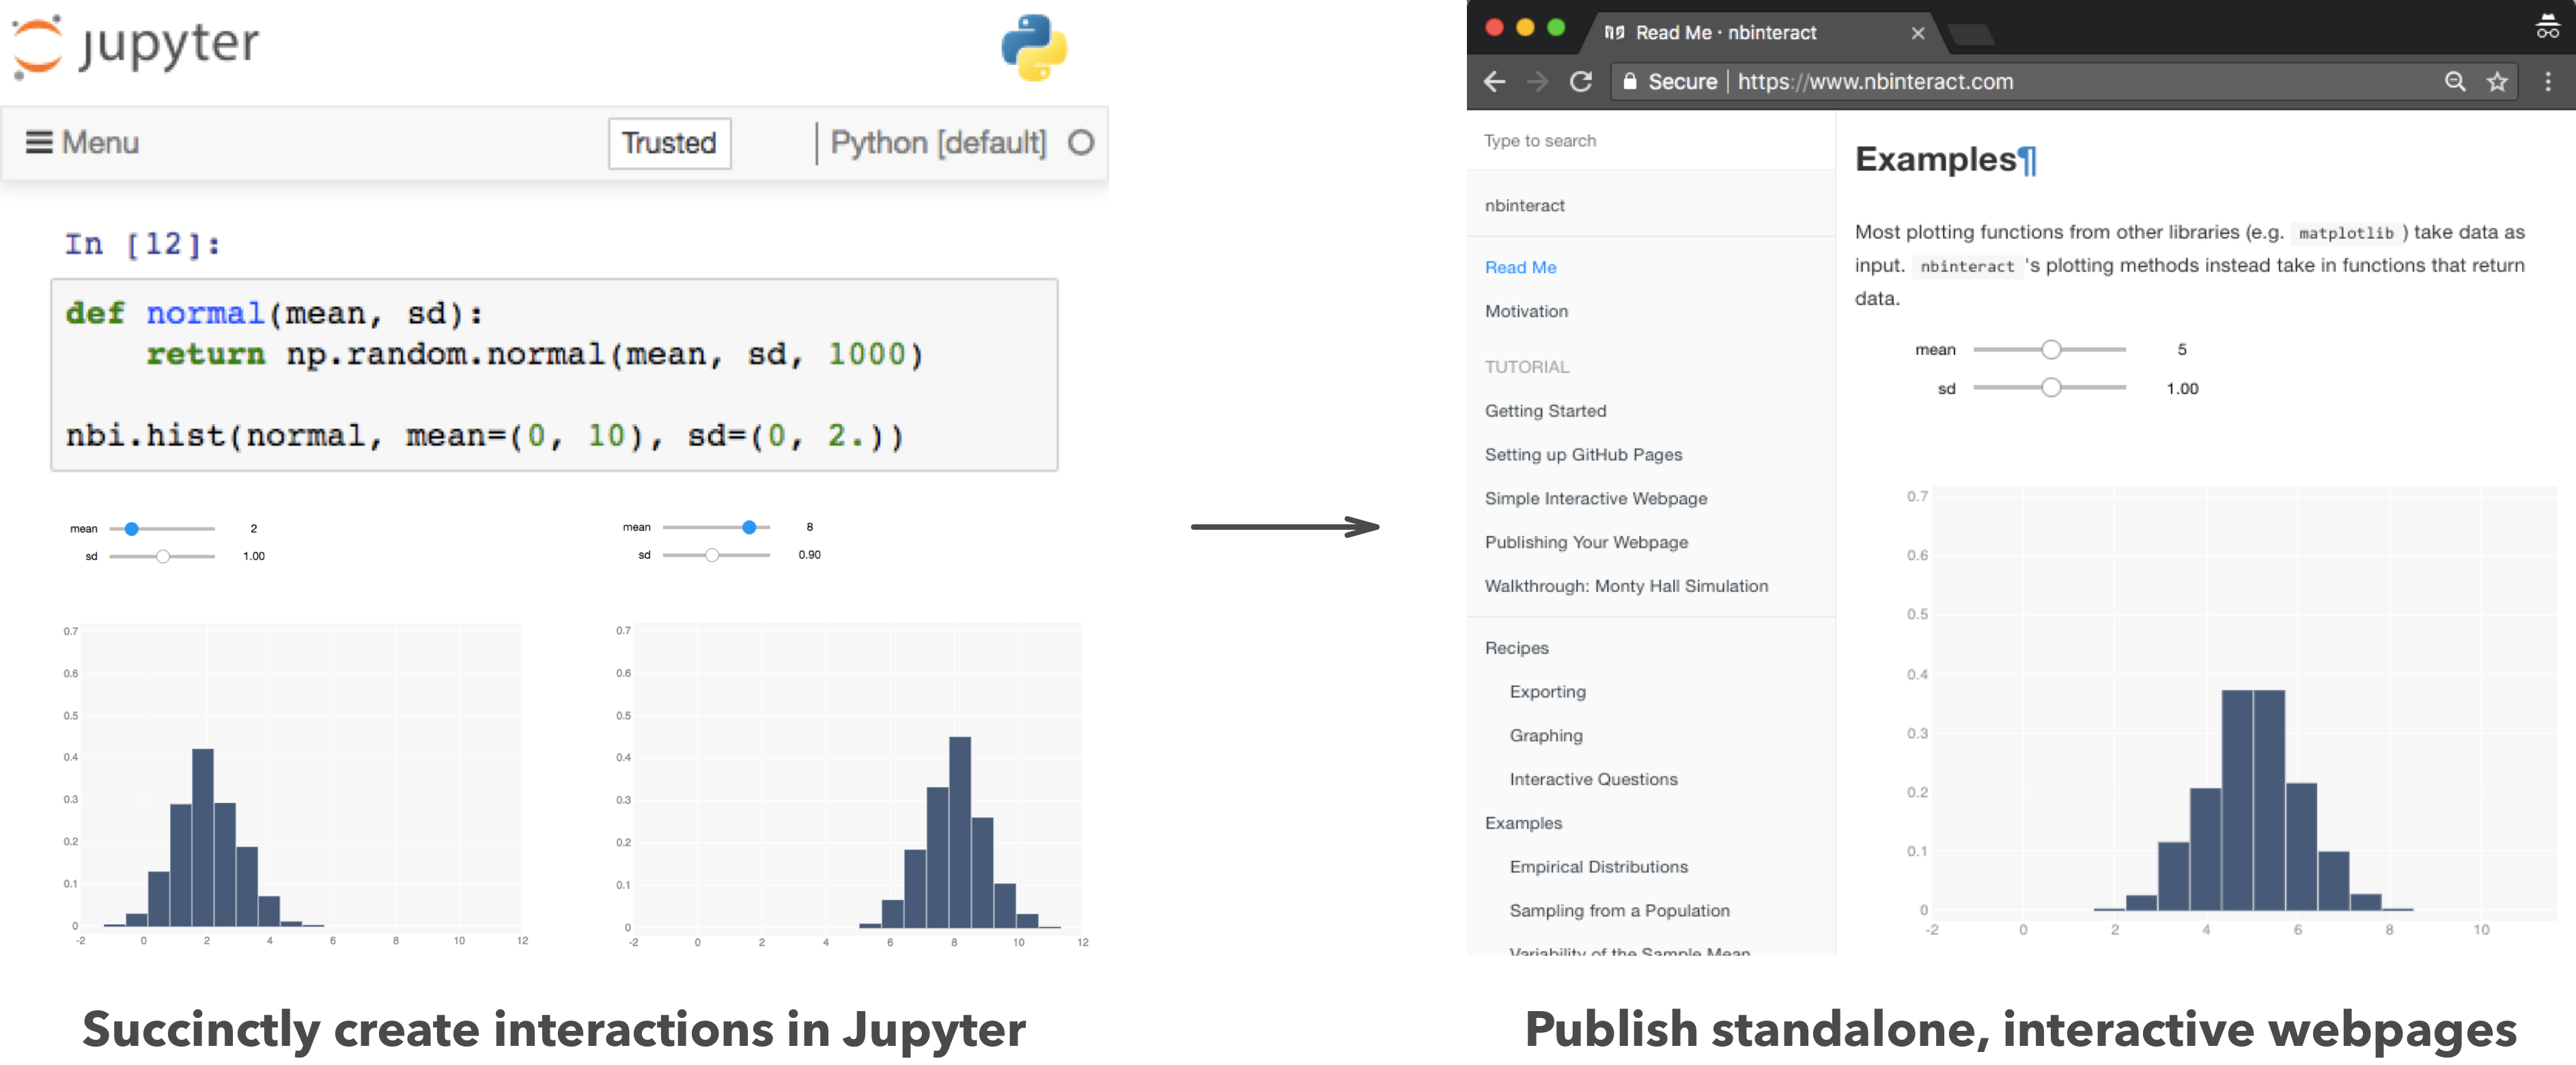
\includegraphics[width=\linewidth]{graphics/cover.png}
  \label{fig:cover}
\end{figure*}

\begin{abstract}
\noindent
\code{nbinteract} provides a Python library and a command-line tool to convert
Jupyter notebooks to standalone, interactive HTML web pages. These web pages
may be viewed by any web browser running JavaScript, regardless of whether the
viewer has Python or Jupyter installed locally. \code{nbinteract}'s built-in
support for function-driven plotting makes interactive visualizations simpler
to create by allowing authors to focus on declarative data changes instead of
callbacks. \code{nbinteract} has use cases for data analysis, visualization,
and especially education, where it is used for a prominent textbook on data
science.
\end{abstract}

\section{Introduction} % (fold)
\label{sec:introduction}

Jupyter notebooks provide a popular document format for authoring, executing,
and publishing code alongside analysis \cite{thomas_jupyter_2016}. Although
Jupyter notebooks were originally designed for use in scientific workflows for
data preparation and analysis, they are becoming an increasingly common choice
for university courses---a survey in 2016 reported that over one hundred
courses across multiple countries use Jupyter in their course content
\cite{hamrick_2016_2016}.

\begin{marginfigure}%
  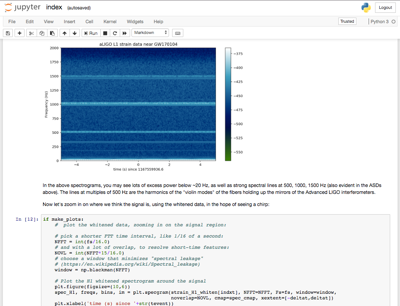
\includegraphics[width=\linewidth]{graphics/jupyter.png}
  \caption{Jupyter notebooks combine code, text, and plots in a single
  document.}
  \label{fig:jupyter}
\end{marginfigure}

An increasing number of universities now offer data science courses, many of
which use Jupyter because of its broad adoption for data analysis workflows in
both academia and industry. These courses often use Jupyter notebooks as the
preferred medium for homeworks, labs, projects, and lectures. UC Berkeley's
flagship data science courses serve thousands of students every year and use
Jupyter for all of these course components.

As a web technology, Jupyter notebooks also provide a platform for interaction
authoring. For example, the popular \code{ipywidgets} Python library allows
users to create web-based user interfaces to interact with arbitrary Python
functions. Users can create these interfaces using Python directly in the
notebook environment instead of having to use HTML and JavaScript,
significantly lowering the time usually needed to create these interfaces
\cite{_jupyter-widgets/ipywidgets_}. This ease-of-use encourages instructors
and researchers to create interactive explanations of their work.

\begin{marginfigure}%
  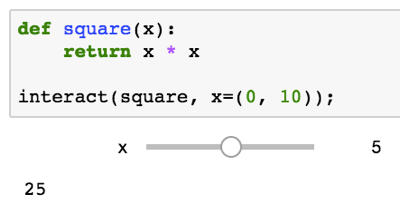
\includegraphics[width=\linewidth]{graphics/ipywidgets.png}
  \caption{The \code{ipywidgets} library provides primitives for interaction
  in Jupyter notebooks.}
  \label{fig:ipywidgets}
\end{marginfigure}

Unfortunately, it is difficult to share these interactive notebooks with the
public. Sharing the notebook file itself retains full interactivity but
requires viewers to have Jupyter, Python, and all other packages used in the
notebook installed on their own machines. The freely available Binder service
circumvents this by hosting notebook servers that come pre-packaged with
necessary software. However, both of these options still require viewers to
have prior familiarity with the Jupyter environment, making them less suitable
for use with non-technical viewers. Authors can convert a Jupyter notebook to a
static HTML document and host the document as a publicly-accessible web page.
However, this method does not preserve the interactive elements of the
notebook; the resulting web page only contains text and images.

\code{nbinteract} is a Python package that allows authors to convert Jupyter
notebooks into interactive, standlone HTML pages. The interactive elements can
use arbitrary Python code to generate output, including Python libraries that
use C extensions (e.g. \code{numpy} and \code{pandas}) and libraries that
create images (e.g. \code{matplotlib}). The resulting web pages can be used by
anyone with a modern web browser even if the viewer does not have Python or
Jupyter installed on their computer. The \code{nbinteract} package also
includes specialized methods for interactive plots designed for fast
interaction prototyping in the notebook and smooth interaction on static HTML
web pages. We discuss the design of the package, its features and limitations,
and its implications for interaction authoring and sharing.

% section introduction (end)

\section{Related Work} % (fold)
\label{sec:related_work}

\subsection{Jupyter Technologies} % (fold)
\label{sub:jupyter_technologies}

The Jupyter notebook platform provides an environment to author code, images,
and written explanations together in a single document composed of multiple
cells. The platform is composed of two main components. It includes a
frontend---a web-based authoring environment that users open in their web
browsers. The frontend connects to a Jupyter kernel, a process on the users'
computers that runs code and returns the output to the frontend to display
\cite{thomas_jupyter_2016}.

The \code{ipywidgets} library makes use of Jupyter's web-based frontend to
create interactive elements directly in the notebook. The library includes
Python functions that produce HTML and JavaScript to display interactive
widgets. When a user interacts with a widget---selecting an option from a
dropdown menu, for example---the \code{ipywidgets} library executes
user-defined Python functions on the Jupyter kernel and renders the result in
the cell \cite{_jupyter-widgets/ipywidgets_}. A number of other specialized
libraries are built on top of \code{ipywidgets}, such as the interactive
plotting library \code{bqplot} \cite{_bqplot_2018} and the molecular
visualization library \code{nglview} \cite{_arose/nglview_}.

Jupyter notebooks use the \code{nbconvert} tool to convert between notebook
formats. \code{nbconvert} also allows notebooks to be converted to static HTML
pages \cite{_jupyter/nbconvert_}. However, these pages do not retain widget
functionality because they do not have access to a Jupyter kernel by default.

The Binder project hosts ephemeral Jupyter notebook servers as a free service
for the general public. It takes a repository of Jupyter notebooks, starts a
Jupyter frontend and Jupyter kernel, and gives users the ability to run the
notebook over the internet instead of having on their local machines
\cite{_binder_}.

\begin{marginfigure}%
  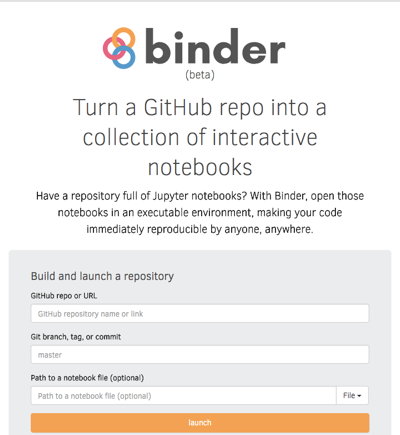
\includegraphics[width=\linewidth]{graphics/binder.png}
  \caption{The free \code{Binder} service runs Jupyter servers for public use.}
  \label{fig:binder}
\end{marginfigure}

% subsection jupyter_technologies (end)

\subsection{Interaction Authoring in JavaScript} % (fold)
\label{sub:interaction_authoring_in_javascript}

JavaScript is the most commonly used language to design interactions that run
in a web browser. Because most modern web browsers run JavaScript natively,
viewers do not have to install additional software in order to make use of
these interactive elements, a key advantage of the language. A number of
authors use JavaScript to create interactive articles
\cite{_explorable_,kunin_seeing_} and textbooks \cite{stark_sticigui_2004}.

There are a number of JavaScript libraries that provide higher level
abstractions for interaction creation such as D3 and Tangle
\cite{bostock_d$3$_2011,bret_tangle_2018}. Fundamentally, most JavaScript
libraries require fluency with aspects of web programming such as JavaScript
syntax and the document-object model. This additional requirement makes
JavaScript more difficult to use for many data scientists; most data science
analysis uses Python and R rather than JavaScript.

The Vega project provides a promising alternative to directly using Javascript
for interaction data visualizations. By defining a grammar of visualization and
interaction, Vega and its ecosystem of projects allow users to declaratively
generate plots that support filtering, panning and zooming. Since Vega
prespecifies available interaction types, however, it does not allow arbitrary
user-defined code to run in response to interaction
\cite{satyanarayan_reactive_2016}.

% subsection interaction_authoring_in_javascript (end)

% section related_work (end)

\section{Features} % (fold)
\label{sec:features}

\subsection{Installation} % (fold)
\label{sub:installation}

Installing \code{nbinteract} requires Python version 3.4 or higher. To install
\code{nbinteract}, run the following command in the terminal:

\begin{verbatim}
  pip install nbinteract
\end{verbatim}

If the Jupyter \code{notebook} package version is lower than 5.3, run these two
additional commands to enable \code{nbinteract} in the notebook environment:

\begin{verbatim}
  jupyter nbextension enable --py --sys-prefix widgetsnbextension
  jupyter nbextension enable --py --sys-prefix bqplot
\end{verbatim}

After installation, the \code{nbinteract} package is available to import in a
Python program and a \code{nbinteract} command-line tool is available to use on
the terminal.

% subsection installation (end)

\subsection{Preparing Notebooks for nbinteract} % (fold)
\label{sub:preparing_notebooks_for_nbinteract}

The simplest method to prepare notebooks for conversion using \code{nbinteract}
is to place the notebooks in a GitHub repository with a \code{requirements.txt}
file in the root directory. The \code{requirements.txt} file should contain all
packages required to run the notebooks. These steps will prepare the GitHub
repository for use on the Binder service, a prerequisite for \code{nbinteract}.
For additional configuration options, consult the Binder
documentation\sidenote{\url{http://bit.ly/binder-docs}}.

% subsection preparing_notebooks_for_nbinteract (end)

\subsection{Command-line API} % (fold)
\label{sub:command_line_api}

\code{nbinteract} provides a command line tool to convert Jupyter notebook
files to HTML files. It requires that a GitHub repository with the notebooks is
set up for use with the Binder service. To convert a notebook to HTML, run the
following command in a terminal shell:

\begin{verbatim}
  nbinteract {owner}/{repo}/{branch} {notebook_name}
\end{verbatim}

Where \code{\{owner\}}, \code{\{repo\}}, \code{\{branch\}}, and
\verb|{notebook_name}| are replaced with the repository's owner, repository
name, branch containing the files, and the name of the notebook to convert. For
example, to convert a notebook called \code{hello.ipynb} residing on the
default \code{master} branch of \code{https://github.com/SamLau95/nbinteract},
run:

\begin{verbatim}
  nbinteract SamLau95/nbinteract/master hello.ipynb
\end{verbatim}

This command creates a \code{hello.html} file using the original
\code{hello.ipynb} notebook. The resulting HTML file may be
uploaded to the World Wide Web using any hosting service, including the free
GitHub Pages service\sidenote{\url{https://pages.github.com/}}.

% subsection command_line_api (end)

\subsection{Python API for Notebook Conversion} % (fold)
\label{sub:python_api}

As a convenience, \code{nbinteract} also provides a Python interface to convert
notebooks to HTML files. To use Python to convert the \code{hello.ipynb}
notebook mentioned above, run:

\begin{minted}{python}
  import nbinteract as nbi
  nbi.publish('SamLau95/nbinteract-image/master', 'hello.ipynb')
\end{minted}

This Python code performs the same conversion as the shell command above.

% subsection python_api (end)

\subsection{Python API for Interactive Plotting} % (fold)
\label{sub:python_api_for_interactive_plotting}

The \code{nbinteract} Python package provides a set of plotting methods for
generating visualizations controlled by interactive widgets. While most
plotting methods in other visualization libraries (e.g. \code{matplotlib}) take
data as input, the plotting methods in \code{nbinteract} take in functions that
generate data as input. For example, the following code generates an
interactive histogram shown in figure \ref{fig:nbi-hist} where the user can
change the mean and spread of a normal distribution:

\newpage

\begin{marginfigure}%
  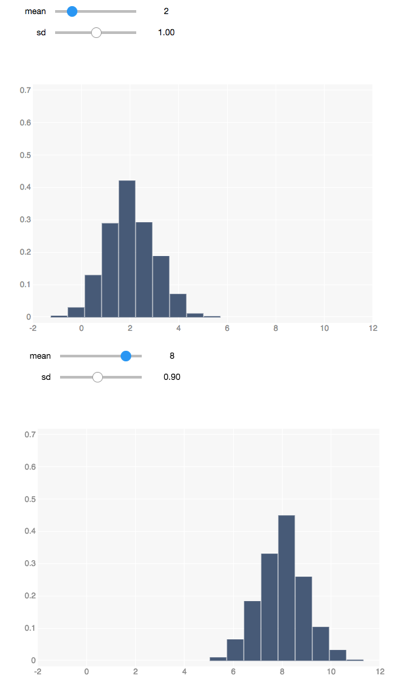
\includegraphics[width=\linewidth]{graphics/nbi-hist.png}
  \caption{The \code{nbinteract} plotting functions create visualizations with
  interactive widgets. Here, two different histogram states are shown.}
  \label{fig:nbi-hist}
\end{marginfigure}

\begin{minted}{python}
import numpy as np
import nbinteract as nbi

def normal(mean, sd):
    '''Returns 1000 points drawn at random fron N(mean, sd)'''
    return np.random.normal(mean, sd, 1000)

# Pass in the `normal` function and let user change mean and sd.
# Whenever the user interacts with the sliders, the
# `normal` function is called and the returned data are plotted.
nbi.hist(normal, mean=(0, 10), sd=(0, 2.0), options=options)
\end{minted}

The plotting methods in \code{nbinteract} take in functions as input and use
the function signature to generate widgets placed above the resulting
visualization. The complete plotting API is documented on \code{nbinteract}'s
website: \url{http://nbinteract.com/}.

% subsection python_api_for_interactive_plotting (end)

% section features (end)

\section{Implementation} % (fold)
\label{sec:implementation}

\subsection{Interactivity for Generated HTML Pages} % (fold)
\label{sub:interactivity_for_generated_html_pages}

Using the base \code{nbconvert} library to convert notebooks to HTML results in
a static HTML page that includes code, text, and images. If the notebook uses
\code{ipywidgets} library to generate widgets, the HTML page also renders
static widgets. Although these widgets respond to user interaction, since the
page does not have access to a Jupyter kernel the widgets will not generate new
output\sidenote{For example, \href{
http://ipywidgets.readthedocs.io/en/stable/examples/Using\%20Interact.html}{
the \code{ipywidgets} documentation} has widgets embedded in the page that are
detached from their original Python output.}.

When a notebook is converted to HTML using \code{nbinteract}, the library
replaces all static widgets with ``Run Widget'' buttons and embeds an
additional JavaScript library in the page. When a ``Run Widget'' is pressed,
the JavaScript library starts a Jupyter kernel using the publicly available
Binder service. Once a kernel is available, the JavaScript library runs the
code on the page and renders live widgets for each cell that originally
generated widgets. The library also handles future communication between the
widgets on HTML page and the kernel so that interacting with the widgets also
updates the output in the HTML. Connecting to a live Jupyter kernel using the
Binder service allows the static HTML page generated from a notebook to contain
dynamic elements.

The JavaScript library for \code{nbinteract} called \code{nbinteract-core} is
publicly available on the JavaScript package
registry\sidenote{\url{https://www.npmjs.com/}} but is neither designed for
general use nor documented on the \code{nbinteract} website.
\code{nbinteract-core} combines three existing APIs in order to enable widget
rendering for static HTML pages: the Binder Web API, the JupyterLab Services
JavaScript API, and the \code{ipywidgets} JavaScript API.

The Binder Web API allows other programs to start Jupyter servers on the Binder
service. Although it is undocumented, the code repository contains an example
of API usage\sidenote{\url{http://bit.ly/binder-api}} which we use to
implement \code{nbinteract-core}.

The JupyterLab Services API contains methods to start and manage Jupyter
kernels on a Jupyter server\sidenote{
\url{https://www.npmjs.com/package/@jupyterlab/services}}. After
starting a Jupyter server using the Binder API, \code{nbinteract-core} uses the
JupyterLab Services API to start a Jupyter kernel in order to run Python code
on the HTML page.

When running code that generates widgets, the \code{nbinteract-core} library
uses the \code{ipywidgets} JavaScript API for rendering the widgets onto the
page\sidenote{\url{https://github.com/jupyter-widgets/ipywidgets}} and sets up
the necessary connection between widgets and kernel so that future interactions
with the widgets will generate new output.

% subsection interactivity_for_generated_html_pages (end)

\subsection{Interactive Plotting Implementation} % (fold)
\label{sub:interactive_plotting_implementation}

\code{nbinteract} combines the \code{ipywidgets} widget library and the
\code{bqplot}\sidenote{\url{https://github.com/bloomberg/bqplot}} plotting
library to implement function-driven interfaces to interactive plotting. The
\code{nbinteract} plotting methods use \code{ipywidgets} to generate and
display widgets, inferring the widget type as needed. When a user interacts
with a widget, a Python callback updates the visualization without a complete
rerender. This noticeably lowers visualization update time compared to using
\code{ipywidgets} alone to render static images.

% subsection interactive_plotting_implementation (end)

% section implementation (end)

\section{Discussion} % (fold)
\label{sec:discussion}

\subsection{Use Cases} % (fold)
\label{sub:use_cases}

Because \code{nbinteract} is designed for use with the Python programming
language in Jupyter notebooks, it provides the most utility for users with
prior familiarity with Python and Jupyter. These users include course staff for
computer science or data science courses, students in these courses, and online
blog authors that use Jupyter notebooks for written content. \code{nbinteract}
can also be used to create dashboards from Jupyter notebooks by hiding the
code used to generate widgets. Since Jupyter notebooks converted to HTML are an
increasingly popular format for online content\sidenote{The first detection of
gravitational waves and Peter Norvig's pytudes are recent high-profile examples
of notebooks used as online content formats.}, we've designed \code{nbinteract}
to easily fit into existing notebook publishing workflows.

UC Berkeley's upper division data science course Data 100 uses
\code{nbinteract} to build its online textbook\sidenote{
\url{https://www.textbook.ds100.org/}}. The textbook is written using Jupyter
notebooks and receives a few hundred views per day. \code{nbinteract} allows
the authors to include interactive widgets anywhere in the textbook. For
example, the book uses widgets to display complete views of large data tables
that would normally require truncation by allowing viewers to scrub through the
rows and columns of the data table as shown in figure \ref{fig:df-interact}.
The book also allows viewers to interactively change parameters and data of
statistical models and displays updated visualizations in response.

\begin{marginfigure}%
  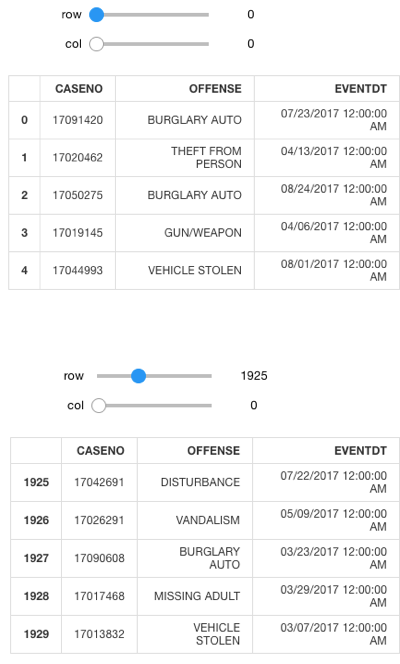
\includegraphics[width=\linewidth]{graphics/df-interact.png}
  \caption{Use of \code{nbinteract} to embed large tables in the Data 100
  Textbook.}
  \label{fig:df-interact}
\end{marginfigure}

% subsection use_cases (end)

\subsection{Comparison with JavaScript} % (fold)
\label{sub:comparison_with_javascript}

Compared to JavaScript, \code{nbinteract} gives authors lower flexibility and
fidelity in exchange for easier interaction creation.

Since web browsers run JavaScript natively, JavaScript users have almost
complete control over every element of the interaction, including the visual
appearance of interactive elements and animations. \code{nbinteract}, however,
limits interactions to the widgets supported by the \code{ipywidgets} and
\code{bqplot} libraries.

Compared to \code{nbinteract}, JavaScript-based interactions will typically
have a lower startup time and a lower latency between user interaction and
visual change. In order to display an interactive element for the first time,
\code{nbinteract} requests a Jupyter server from the Binder service. This
initial request adds 5-10 seconds to the initial startup time. On user
interaction, \code{nbinteract} runs Python code on a remote Jupyter kernel,
incurring overhead from network latency in addition to the time it takes the
kernel to run the Python code. Typically, interactions can be structured in a
way to minimize code execution time when widgets are manipulated, making
network latency the most significant overhead for user interaction. On fast
connections, this latency is typically around 100 milliseconds.
JavaScript-based interactions, however, typically do not make requests to a
remote server and thus do not incur network latency overhead.

Interactions that both \code{nbinteract} and JavaScript support are typically
easier to create in \code{nbinteract} than in JavaScript. Authors fluent in
Python can often write interactions with an order-of-magnitude fewer lines of
code in \code{nbinteract} than authors fluent in JavaScript. The simplicity of
\code{nbinteract} makes it attractive for authors already knowledgable in
Python but not JavaScript and HTML.

% subsection comparison_with_javascript (end)

\subsection{Future Work} % (fold)
\label{sub:future_work}

Although \code{nbinteract} is not designed to fully replicate the flexibility
and fidelity of JavaScript, we hope to make several improvements to the library
in order to increase utility for authors that use Jupyter notebooks.

We plan to release a more flexible API for creating interactive visualizations
using \code{nbinteract}. Currently, visualizations are restricted to single
plots that contain one type of mark (e.g. line, point, or bar). Our future API
will provide a declarative syntax for connecting multiple widgets, functions,
and plot elements to create more complex interactive visualizations.

Currently, \code{nbinteract} only permits widgets from the \code{ipywidgets}
and \code{bqplot} libraries. Since there are now many libraries built on top of
the \code{ipywidgets} library\sidenote{Any of the widget libraries listed at
\url{http://jupyter.org/widgets}, for example.}, we plan to allow authors to
specify additional widget libraries when converting notebooks. This improvement
will allow \code{nbinteract} to support the entire ecosystem of interaction
frameworks that use \code{ipywidgets}.

We also plan to work with the Binder team to decrease the startup time of
Jupyter servers on Binder. This improvement would benefit both
\code{nbinteract} users and any user of the Binder service itself. We are also
investigating ways to reduce latency after widget initialization, including
caching previous interaction outputs on the client and batching visualization
updates together.

% subsection future_work (end)

% section discussion (end)

\section{Conclusion} % (fold)
\label{sec:conclusion}

\code{nbinteract} combines recently developed projects in the Jupyter ecosystem
to allow authors to create interactive explanations and visualizations directly
in the Jupyter notebook environment. The library aims to use the broad adoption
of Python and Jupyter to allow many more individuals to create and share
interactive content online.

% section conclusion (end)

\newpage

\printbibliography

\end{document}
